%%%%%%%%%%%%%%%%%%%%%%%%%%%
\chapter {Parallel Black Virus Decontamination in Arbitrary Graph}
\label{TL}
%%%%%%%%%%%%%%%%%%%%%%%%%%%

%\color{blue}
%Use $x,y,z$ for indicating nodes, use something different to indicate ``numbers" ($n,m,,k,h ...$).
%\color{black}
\section{Introduction}
In \cite{cai}, Cai proposes two exploration strategies: Greedy Exploration and Threshold Exploration, both spread optimal and total number of agents asymptotical optimal. Since these strategies are sequential, they are time consuming($O(\Delta n^2)$).  In order to explore the graph in parallel, we propose two different strategies: \\
(1) Flood Strategy\\
(2) Castle-First Strategy\\
The general idea of the Flood Strategy is simple: supposing that an agent resides in node $v$, and it has $m$ neighbours  to be explored, then it simply clones $m$ agents and send them to its neighbours. In the Castle-First Strategy, we build ``castles" which are structures composed by  a single node or by a combination of several nodes with special properties (rules are introduced later); the exploration phase can be viewed as the combination of several smaller scale explorations in the graph and it begins with the location of one of the exploring group and ends with one of the unexplored castles. We will see that after all the castles are explored, all the nodes in the graph are explored. The general exploring algorithm for these two strategies is based on the one described in Chapter 3 which consists of performing a {\em Shadowed Exploration} phase to locate the BV, followed by a {\em Surrounding and Elimination} phase to eliminate the cloned BVs. 

Strategy {\em Flood}  is time optimal with the cost of a great number of agents,
 while strategy {\em Castle-First} comes to a compromise between  {\em Flood} and the sequential strategies: it employ much less agents than  {\em Flood} and it costs much less  than the sequential strategies in terms of time. 

\color{blue}In the arbitrary graph, we assume that  the original BV and its clones do not disconnect the graph.
\color{black}
\section{The Flood Strategy}
\noindent{\bf Initialization.}
In this strategy, we assume that all the agents are endowed with 3-hop visibility. For this strategy, in contrast with the sequential strategy, agents   do not need memory to remember the routes they pass by.  Finally, in this strategy, we use an important ability of agents which is ``cloning". As we introduced in Chapter 2, cloning means that an agent is endowed with the capacity to generate one or more agent identical to itself. 

We use the Dijkstra Algorithm to compute the shortest route from the homebase to every node and write the route step on the white board on each node, so for each node, there should be a number (Shortest Route Number) recording the number of steps of the shortest route from the homebase to it. Let us denote by $v_{SRN}$ the Shortest Route Number of node $v$, and nodes ${v_1, \ldots, v_i}$ are neighbours of node $v$ assuming that $v$ has $i$ neighbours. Then edges connecting node $v$ and its neighbours are $e(v, v_1), \ldots, e(v, v_i)$. We write the $v_{SRN}$ in correspondence to the   end port of these edges (the end connecting to its neighbours), so when an agent resides in any node from $v_1$ to $v_i$, it can see the Shortest Route Number of node v because of the local visibility (see, for example,   Fig \ref{fig:Arbi1}).

\begin{figure}[H]
  \centering  
  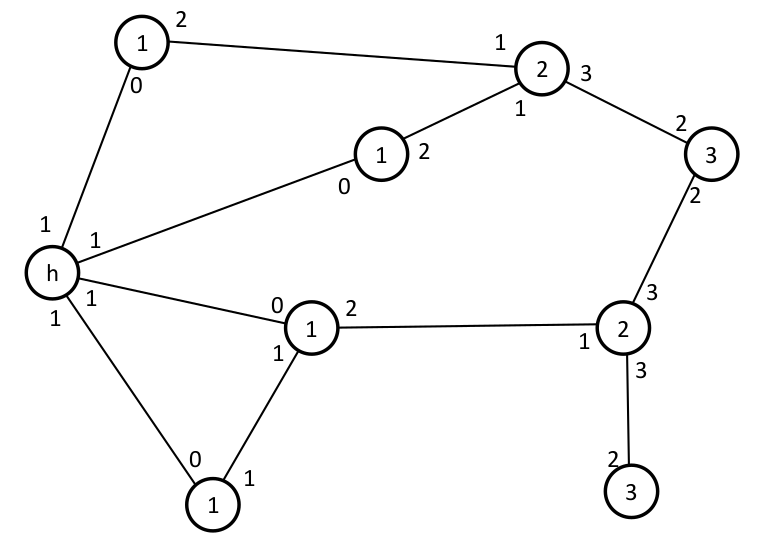
\includegraphics[width=3in]{figures/Arbi1.png}
  \caption{Initialization of the graph}\label{fig:Arbi1}
\end{figure}

\noindent{\bf Exploration Phase}
All the agents in this strategy follow the same rules in the exploration phase.
%Rules for agents in the exploration phase:
Let us denote by $SNR$ the Shortest Route Number.
\begin{enumerate}
\item Agents can only move from node with lower $SNR$ to node with higher $SNR$.
\item Let  $m$ agents reside in node $v$ with   $SNR$ of $v$ equal to $a$, and let  the next destination(s) (node $v$'s neighbours with higher $SNR$ than $v$') be $\{v_1,\ldots, v_k\}$. (such a neighbour always exist)

   %  -   if $m\geq k+1$, then $k$ agents move to the $k$ destinations  while the remaining agents stay in node $v$ to guard $v$ at $T_i$.  If $m< k+1$, then one of the agents residing in node $v$ clones $k+1-m$ agents and 
- if $m<k+1$ (the number of agents is not sufficient), then one of the agents residing in node $v$ clones $k+1-m$ agents. After that, $k$ agents of the agents residing in node $v$ move to the $k$ destinations while the remaining agents stay in node $v$ to guard $v$ at $T_i$. 
 If one of the agents is destroyed, the Elimination phase begins; if none of the agents are destroyed, the remaining $m-k$ agents %\color{blue}  {\bf what do you mean ``randomly???} \color{black} 
move to any of the $k$ destinations at  time $T_{i+1}$. 
 
 \color{blue} are the destination the same as the neighbour ? If indeed the two rules are the same except for the cloning you should put them together saying simply that if the number of agents is not sufficient ($m< k+1$), the necessary number is cloned.  Do not use the term "random", just say move in "any" ....\color{black} \\
     %-   if $m< k+1$, then one of the agents residing in node $v$ clones $k+1-m$ agents, and these $k$ agents move to all the neighbours at $T_i$. If one of the agents is destroyed, the Elimination phase begins; if none of the agents are destroyed, the agent guarding node $v$   moves to one of the neighbours with $SNR$ equal to $a+1$ at time $T_{i+1}$ 
     \color{blue} (such a neighbour always exist). \color{black}
     
%\color{blue}  Wouldn't this happen also in the previous case ?(Yes, but in the first case, no agents should be cloned.  Isn't the next rule part of this (Yes, but in next rule, no agents should be cloned) ?\\  
- If an agent resides in a node without any neighbour whose $SNR$ equal to $a+1$, then it simply stays there.
 \color{black}
        Since all the action of agents happen after they meet each other at the same node, they can communicate with each other and make sure that all their routes do not conflict.
%\item If an agent resides in a node without any neighbour whose $SNR$ equal to $a+1$, then it simply stays there.
% 
%        Since all the action of agents happen after they meet each other at the same node, they can communicate with each other and make sure that all their routes do not conflict.
\end{enumerate}
An example of how the agents move is showed in Fig \ref{fig:Arbiflood}
\begin{figure} [H]
  \centering 
  \subfigure[$T_1$]{ 
    \label{fig:Arbiflood1:a} %% label for first subfigure 
    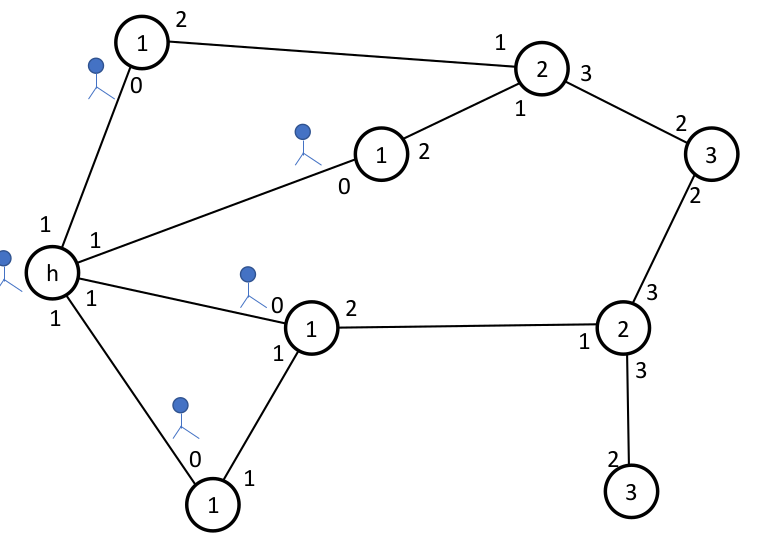
\includegraphics[width=2.5in]{figures/Arbiflood1.png}} 
%  \hspace{1in} 
  \subfigure[$T_2$]{ 
    \label{fig:Arbiflood2:b} %% label for second subfigure 
    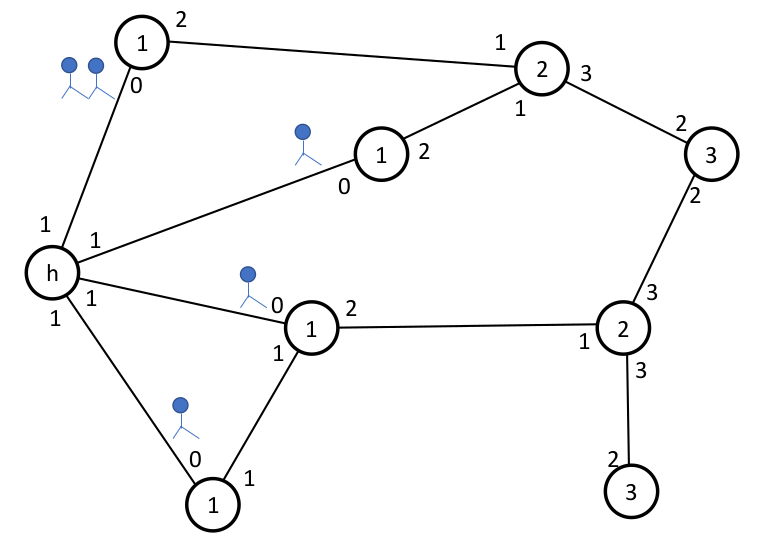
\includegraphics[width=2.5in]{figures/Arbiflood2.png}}
    \hspace{1in} 
  \subfigure[$T_3$]{ 
    \label{fig:Arbiflood3:c} %% label for second subfigure 
    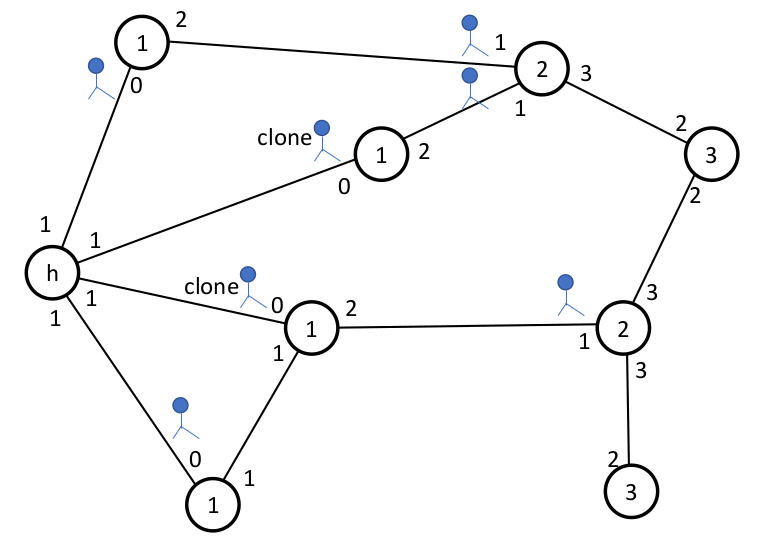
\includegraphics[width=2.5in]{figures/Arbiflood3.png}}
%      \hspace{1in} 
  \subfigure[$T_4$]{ 
    \label{fig:Arbiflood4:d} %% label for second subfigure 
    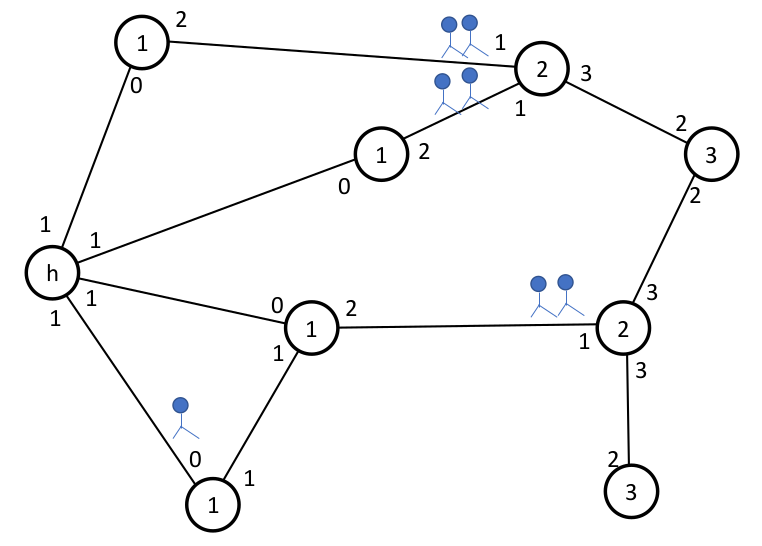
\includegraphics[width=2.5in]{figures/Arbiflood4.png}}
      \hspace{1in} 
  \subfigure[$T_5$]{ 
    \label{fig:Arbiflood5:e} %% label for second subfigure 
    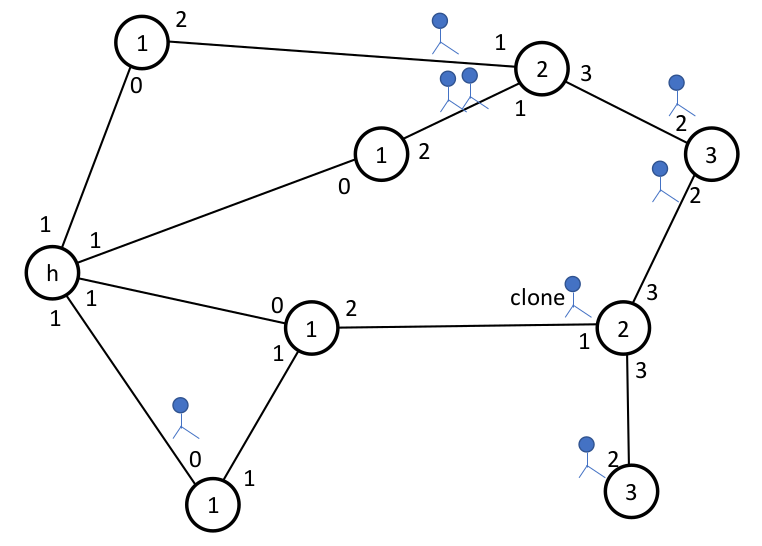
\includegraphics[width=2.5in]{figures/Arbiflood5.png}}
     \subfigure[$T_6$]{ 
    \label{fig:Arbiflood6:e} %% label for second subfigure 
    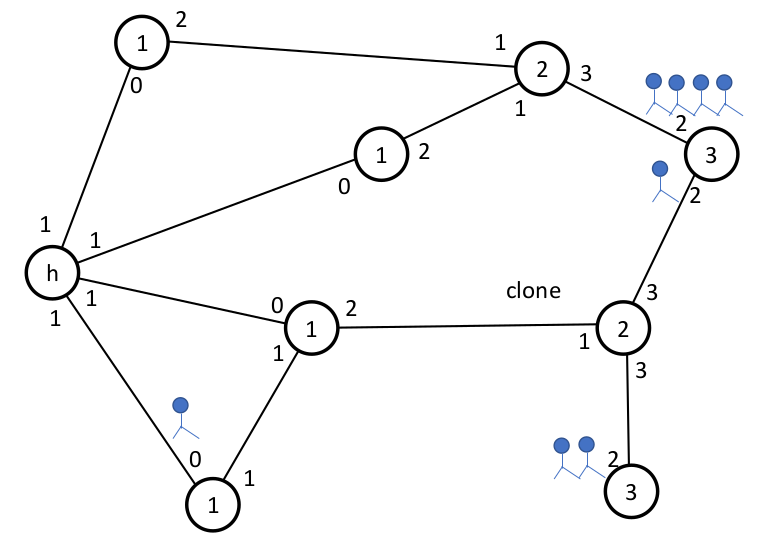
\includegraphics[width=2.5in]{figures/Arbiflood6.png}}
  \caption{An example of how the agents move in the Flood Strategy} 
  \label{fig:Arbiflood} %% label for entire figure 
\end{figure}      

\noindent{\bf Elimination Phase.}
Let us assume that the node where the original BV resides is $v$ with $SNR$ equal to $a$ and that it is triggered at time $T_i$. Then at this time, the clones spread to all neighbours of node $v$ with $SNR$ equal to $a+1$ and survive while leaving node $v$ clean (no agent and no BV) and let us denote by $v_{BV}$s all these BV nodes.  

We now  describe how agents residing in different positions move in the Elimination phase.
\begin{enumerate}

\item Rule 1: For convenience, we call agents residing in the   $v_{BV}$s' neighbours with $SNR$ equal to $a$ the {\em Witness Agents}. Note that the  Witness Agents can easily realize whether or not node $v$ is the place where the original BV resides. In fact, since they have 3-hop visibility, if they see that one of their ``2-distance" neighbours (say node $v'$) does not contains an agent but some neighbours of node $v'$ contain agents, they   know that the original BV resides in node $v$. If the Witness Agents realize the existence of BV at time  $T_i$, then they simply stop cloning and moving to the new formed BV nodes. Note that if the Witness Agents (say it resides at some node $u$) have some higher $SNR$ neighbours except for the new formed BVs, they should still explore these nodes following the rules in the exploration phase but leaving an agent in node $u$ to guard it.  

\item Rule 2: For all of the agents residing in node $v$'s neighbours with $SNR$ equal to $a-1$ (say  there are $k$ such agents), they receive clones and understand the location of the BV,  and should move to $v$ at  time $T_{i+2}$. Let us denote by $p$ the number of $v$'s neighbours with $SNR$ equal to $a+1$, then if $k< p+1$, one of the agents residing in node $v$ should clone another $p+1-k$ agents and then $p$ agents move to $v$'s neighbours with $SNR$ equal to $a+1$ at $T_{i+4}$.
\end{enumerate}

\color{blue} Note that in our assumptions, the original BV and its clones do not disconnect the graph,  so there should be other routes from the homebase to the new BV nodes even excluding   the original BV node. \color{black} So when $z$ agents are sent to $v$'s neighbours with $SNR$ equal to $a+1$ at time $T_{i+4}$, some other agents move to these nodes's higher $SNR$ neighbours at the same time, which ensure that all the neighbours of the new formed BVs are guarded when they are triggered. 

See Fig \ref{fig:BVd}. For convenience of description, we give every node in the graph a distinct ID from 1 to 13. As shown in the picture, when the BV is triggered, the clones spread to all neighbours of node 3;  node 4 and 5 become new BV nodes while nodes 1, 2 and 12 destroy a clone each and understand  that the original BV resides in node 3. 
%
\begin{figure} [H]
  \centering 
  \subfigure[$T_i$]{ 
    \label{fig:BVd1:a} %% label for first subfigure 
    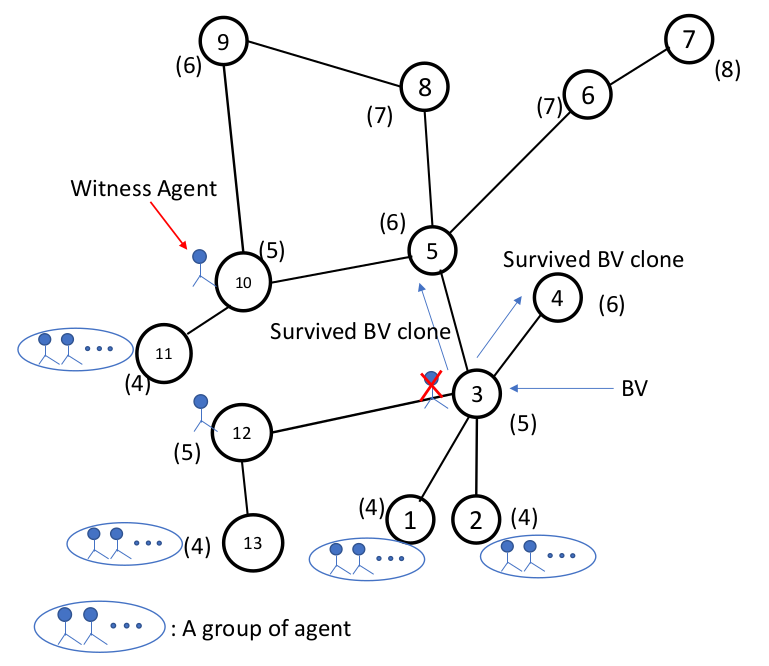
\includegraphics[width=2.5in]{figures/BVd1.png}} 
%  \hspace{1in} 
  \subfigure[$T_{i+1}$]{ 
    \label{fig:BVd2:b} %% label for second subfigure 
    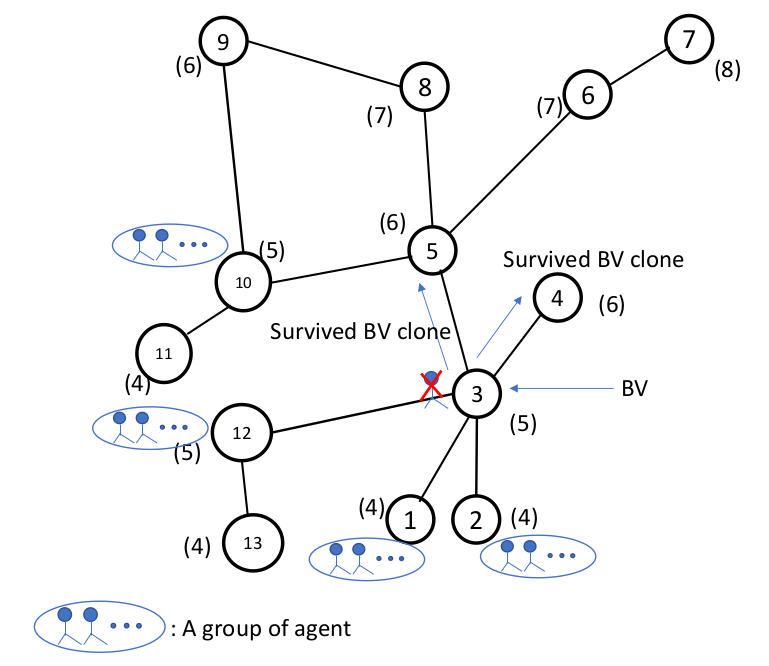
\includegraphics[width=2.5in]{figures/BVd2.png}}
    \hspace{1in} 
  \subfigure[$T_{i+2}$]{ 
    \label{fig:BVd3:c} %% label for second subfigure 
    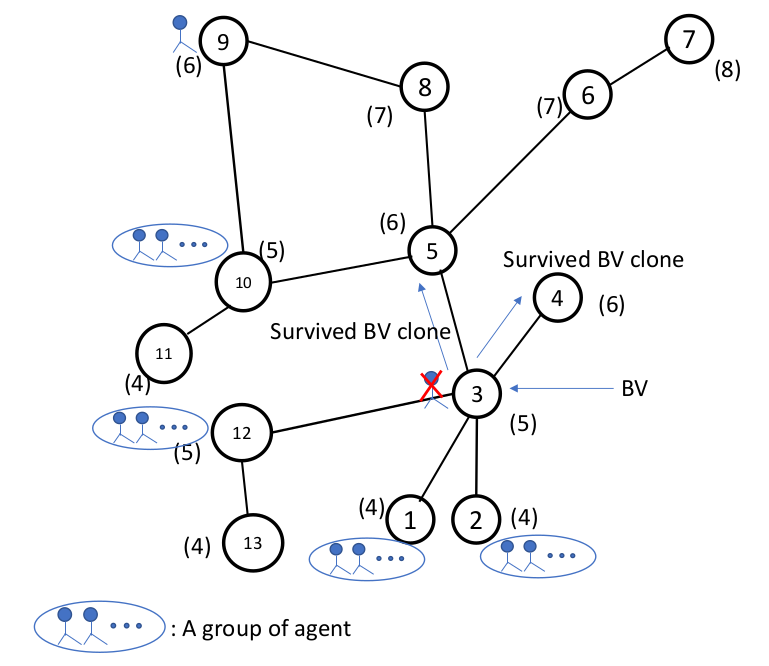
\includegraphics[width=2.5in]{figures/BVd3.png}}
%      \hspace{1in} 
  \subfigure[$T_{i+3}$]{ 
    \label{fig:BVd4:d} %% label for second subfigure 
    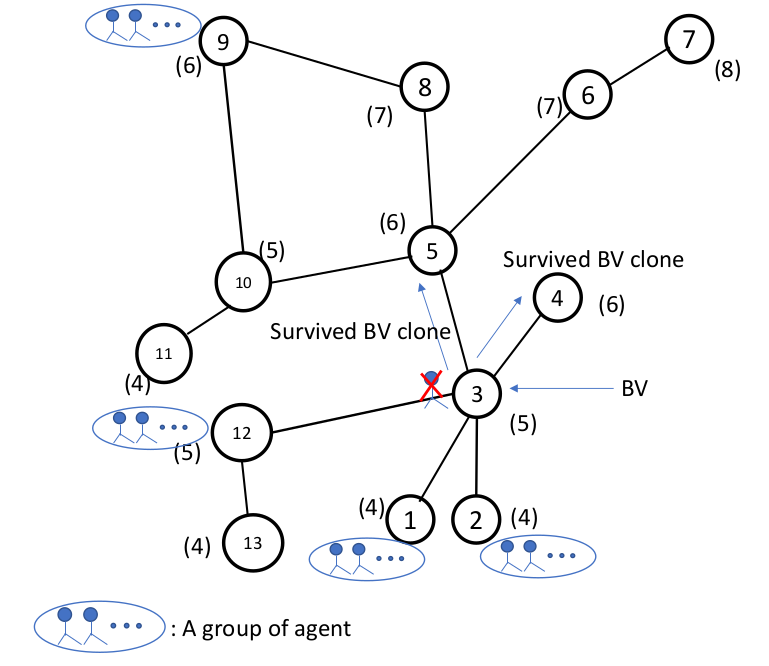
\includegraphics[width=2.5in]{figures/BVd4.png}}
\caption{A possible situation when the BV is detected. The Ids of the nodes are written inside the nodes, their SNR value is indicated in parenthesis.} 
  \label{fig:BVd} %% label for entire figure 
\end{figure}    

 
In Fig. \ref{fig:BVd}, an agent residing in node 10 is a Witness Agent and, because of the 3-hop visibility, it can ``see" that there is no agent residing in node 3 but there are agents residing in node 3's neighbours  (node 1 and node 2). In this way, it knows that the original BV resides in node 3, therefore, it stops moving and cloning towards the BV but,  since it has still   a higher $SNR$ neighbour (node 9) which does not contain a BV,   it continues the exploration in that direction following the rule in the exploration phase. That is, it sends an agent to node 9, then all the agents except one move to node 9. After that, one agent is sent to node 8. 

\begin{theorem}
Let $h$ be  the diameter of the graph. The Flood Strategy performs the exploration phase in  $2h$ unit of time.
\end{theorem}
\begin{proof}
According to the rules in the exploration phase, the agents keep exploring when they have no more higher $SNR$ neighbours, which means the exploration phase ends when the node(s) with the highest $SNR$ is explored and this $SNR$ should be the diameter of the graph. Since exploring nodes with the same $SNR$ requires 2 units of time, the exploration phase needs $2*h$ unit of time.
\end{proof}


%For convenience, let us denote by $a$ the $SNR$ of the original BV node. Since in our assumption, any node does not disconnect the graph, so the following situation would not happen:
%\begin{enumerate}
%\item All the higher $SNR$ neighbours of the new formed BVs have only one neighbour with lower $SNR$ and it is the BV node, \item Some of the neighbours of the new formed BVs have at least one neighbour with lower $SNR$ except their BV neighbour while some of the neighbours of the new formed BVs have only one neighbour with lower $SNR$.
%\end{enumerate}
%For example, see \ref{fig:Arbi3}. The situation shown in the red circle is the case when the node 5 disconnect the graph.The new formed BVs has two higher $SNR$ neighbours which are nodes 8 and 6. Node 6 has only one neighbour with lower $SNR$ and it is the BV node. Assuming the BV is triggered at $T_i$, then at $T_{i+2}$, all the BVs are decontaminated except one: the BV clone spreading to node 6, so we can only employ an agent to move to node 6, then to node 7 and the BV is permanently destroyed and we do not want it to happen.

%With our assumption, all the higher $SNR$ neighbours of the new formed BVs have at least one neighbour with lower $SNR$ except their BV neighbour.  Since agents who do not know the existence of the BV keep moving and at $T_{i+2}$, they would move to occupy nodes with $SNR$ equal to 7 which means all the neighbours of the new formed BV are guarded. In this way, all the BVs are permanently destroyed at $T_{i+2}$.

               
\section{Castle-First Strategy}
\subsection{ Introduction}
In the Castle-First Strategy, all the agents have only   local visibility. But the leader agent in each exploration group has the map of the graph in its memory. Furthermore, the leader agents are endowed with the ability of clone.

In the Castle-First Strategy, we build some castles based on the  $SNR$ of the nodes. More than one group of agents are sent to explore the graph at the same time. Their exploration of the graph is separated into many ``sub-exploration"s and each ``sub-exploration" begins   where a group of  agents are  initially residing  and ends with a new unexplored castle. The map of the graph with all the castles %\color{blue} 

being pointing out is recorded on the whiteboard on nodes with more than two neighbours (called the {\em intersections}) so when agents move across these nodes, they can update the information on the whiteboard (for example, changing the state of some castles into explored and update its own memory %(explanation : the updated information should be viewed by other agents so they should change the state. they cannot only change their own memory)
When agents cannot find an unexplored castle in the graph,  they terminate. 

\subsection{ Initialization}
Based on the graph marked $SNR$ for every node, we built another graph called ``Castle Graph". 
We now give the definition of ``Castle":
\begin{definition}
\noindent (1): A node with a single neighbour is a Castle.
\noindent (2): A group of connected nodes with the same $SNR$  is a Castle;
\noindent (3): A node with more than two neighbours with lower $SNR$ than itself, is  a Castle.
\end{definition}
 

%1. Case 1: Node who has one neighbour is a ?Castle?.
%2. Case 2: If a node has at least one neighbour with the same SNR as it, then the combination of them is a castle. If different castles have at least one common node, then we merge them into a bigger castle;
%3. Case 3: If a node has more than two neighbours with lower SNR than itself, than this node is a castle.
Some examples of castles are shown in Fig  \ref{fig:CastleExample}
\begin{figure}[H]
  \centering  
  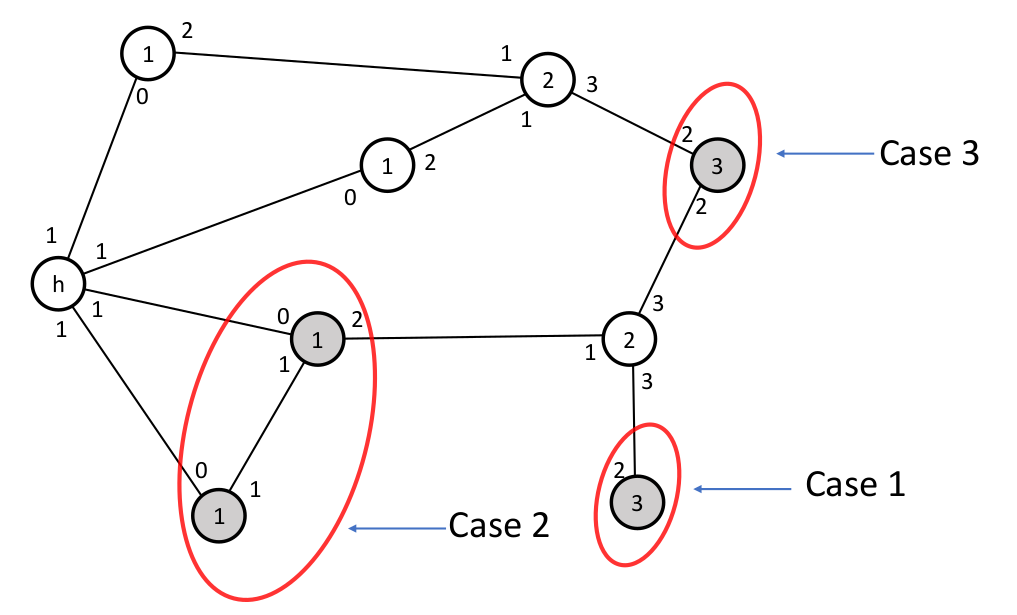
\includegraphics[width=3.5in]{figures/CastleExample.png}
  \caption{Examples of Castles}\label{fig:CastleExample}
\end{figure} 

After the processing, we have a new graph called ``Castle Graph", and a ``Castle Graph" is a graph with the indication of all the castles positions. This graph is presented on the whiteboard on the nodes which have more than two neighbours, so when the agent reaches this node, it can read the graph to update its own information or using its own information to update the ``Castle Graph". 

%\color{blue} (I add the explanation above)
%Not clear what is a castle graph. Just the indication of the castles positions  or the subgraph induced by them ?   \color{black}

\subsection{ Exploration Phase}
The Exploration Phase of the Castle-First Strategy is shown in Fig \ref{fig:castlestates} 
%\color{blue} wrong figure ? \color{black} 
and is introduced in detail in the following.
\begin{figure}[H]
  \centering  
  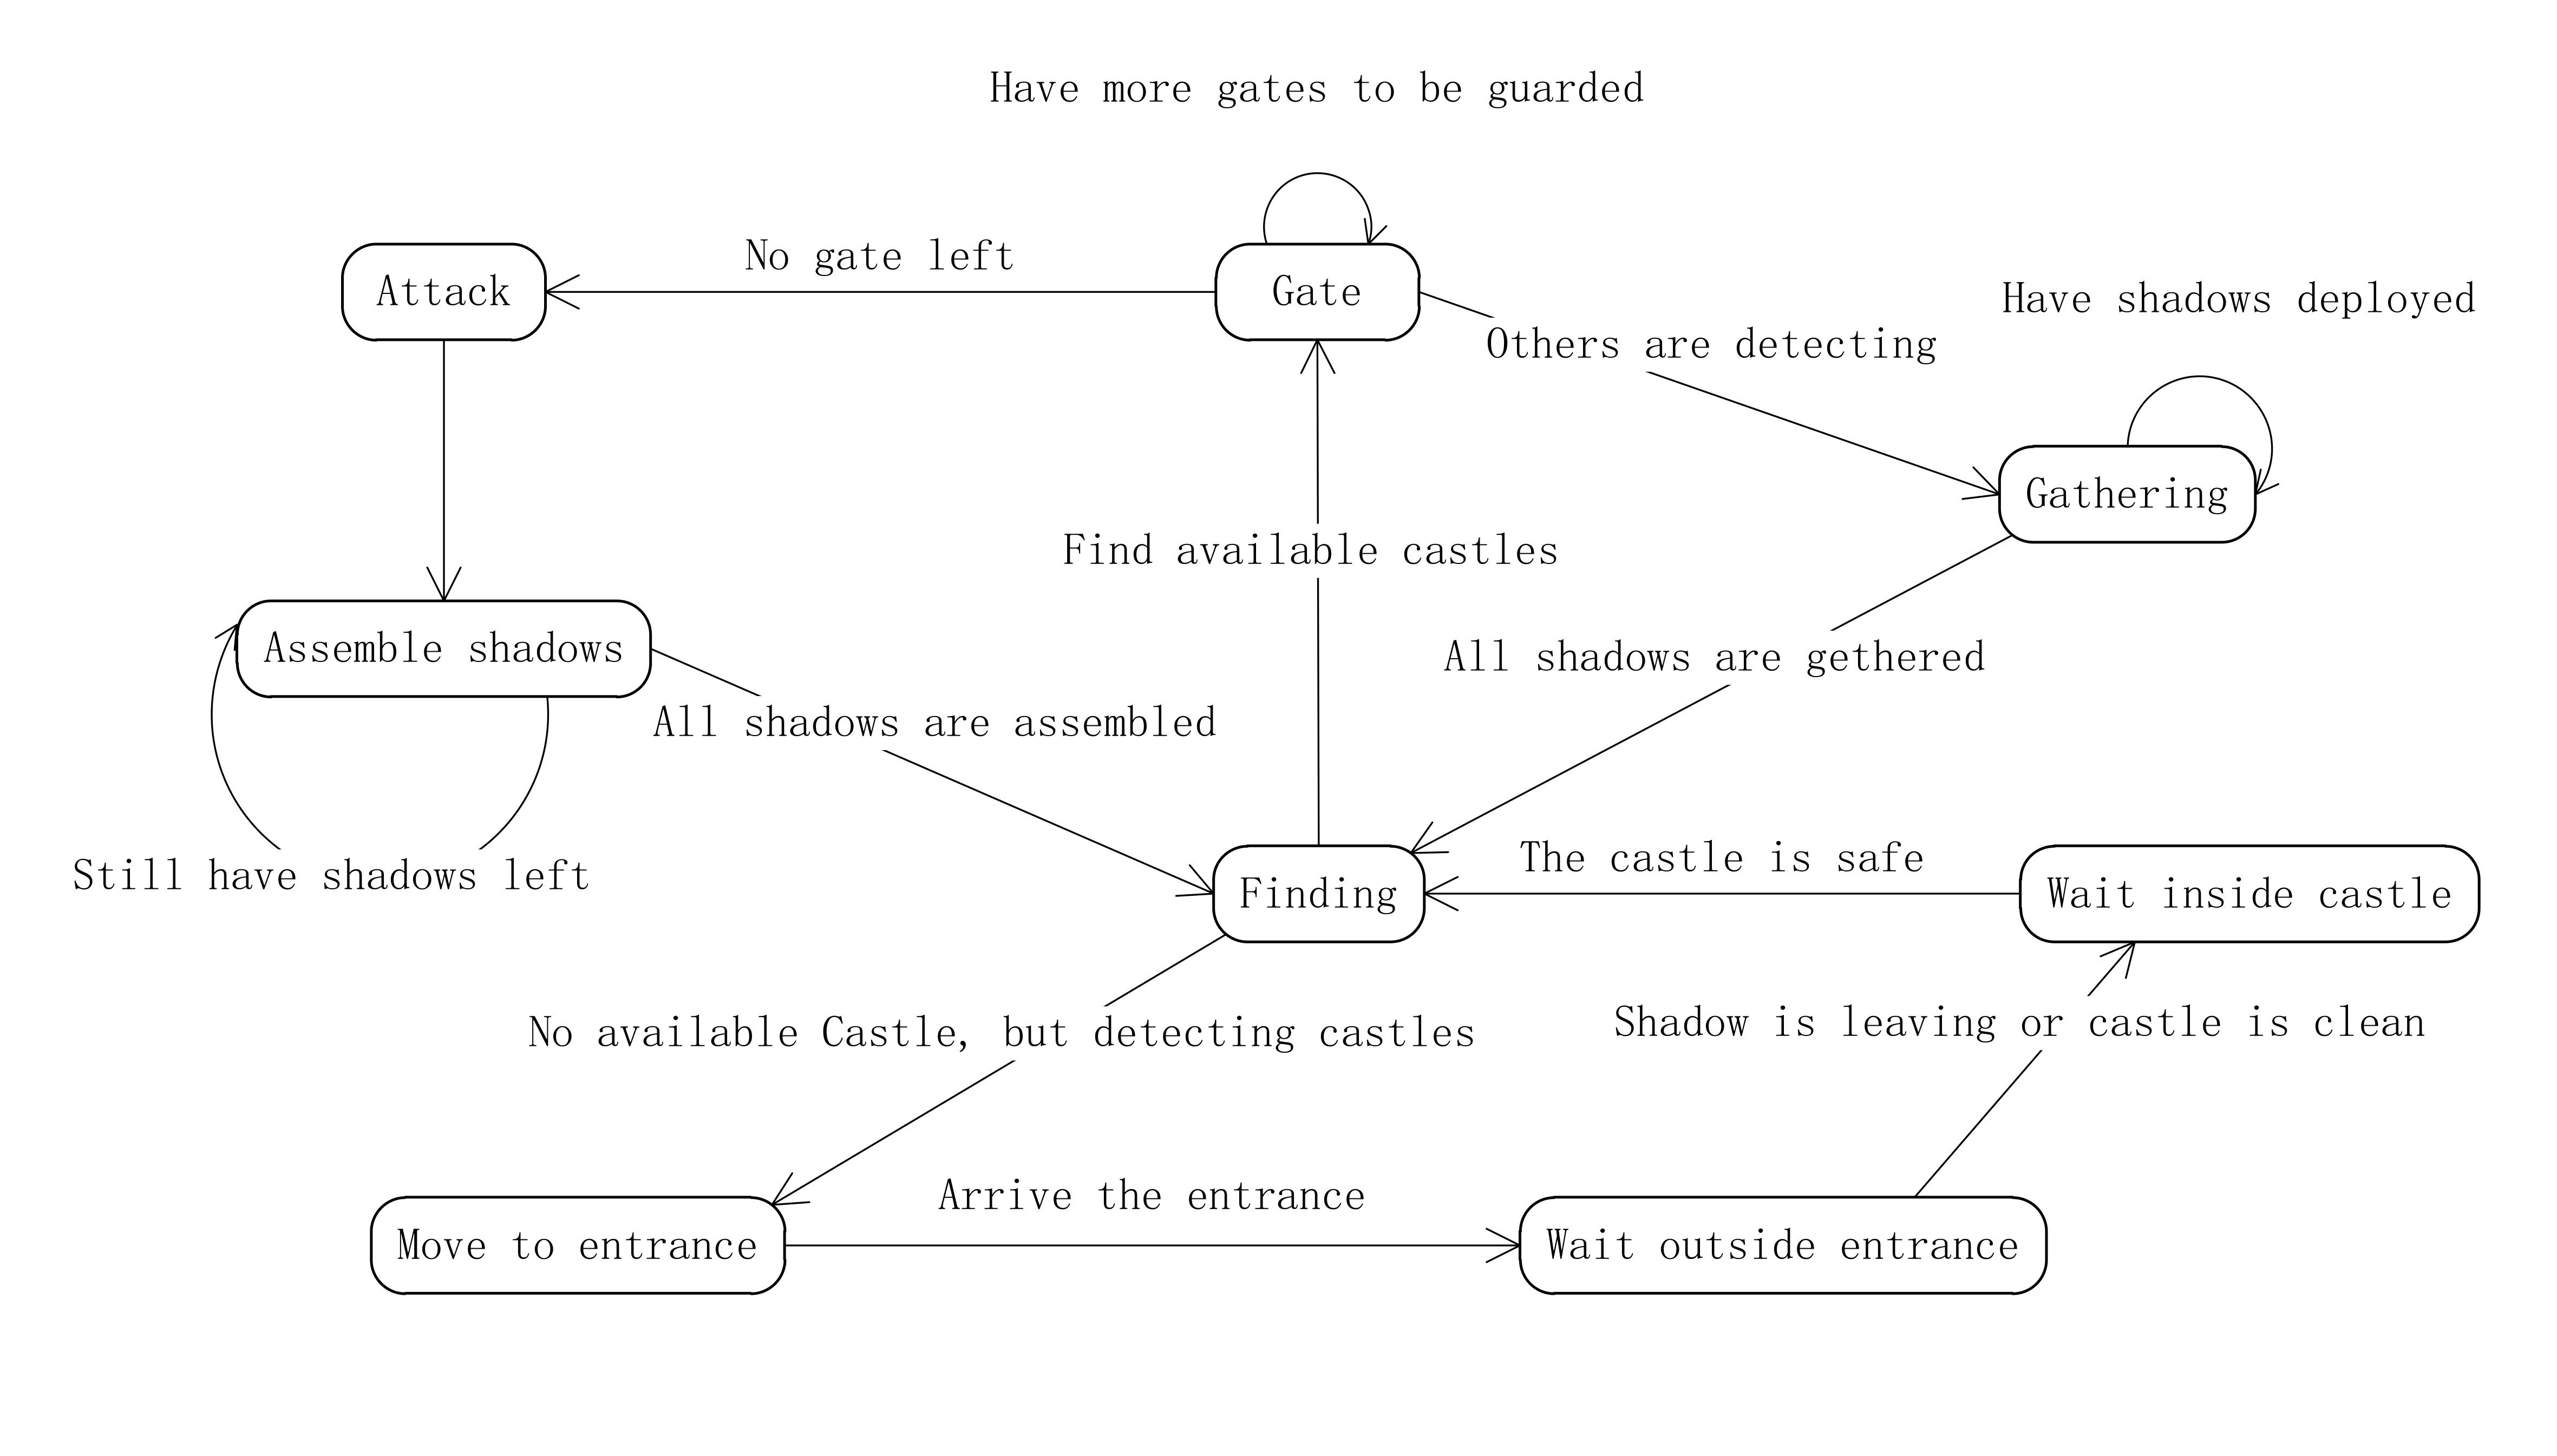
\includegraphics[width=6.0in]{figures/castlestates.png}
  \caption{Exploration phase of the Exploration Phase}\label{fig:castlestates}
\end{figure} 
 
There are two principles in the exploration phase for the agents:
\begin{enumerate}
\item When agents move in an unexplored area, they should strictly move from node with smaller $SNR$ to node with bigger $SNR$ and should follow the cautious walk; on the other hand,  when they move in an explored area, they can move in  any direction   (so, also from bigger $SNR$ to smaller $SNR$) and when they  move in this area, they  do not do it with cautious walk  (for example, when they plan to explore node $v$ from node $u$, the LA can directly move to node $v$ when node $v$ is in the explored area), which is called ``normal walk".
\item The castle ${\cal C}$ selected to be the destination of the ``sub exploration" should meet  the following requirement: assuming that the $SNR$ of ${\cal C}$ is $a$ and 
that the agents start the  ``sub exploration" from node  $v$, 
 then for every node $w$ with $SNR$ equal to $a-1$ connected to {\cal C}, there should be a route from   $v$ to $w$    and no other unexplored or ``under-exploration" castle(s)  should exist on these routes. In another word, when the agents move from $v$ to one of these nodes,   they do not  need to ``attack" other castles. 
\end{enumerate}  

There are two kinds of agents in this strategy: {\em Leader Agents} (LA) and {\em Shadow Agents} (SA) and the LA has the map of the whole graph in its memory. When more agents are needed, the LA can clone the necessary agents. At the beginning of the exploration phase, the LAs are in the homebase, so they each pick a different castle to be the destination of the their first ``sub exploration" and since they have the map of the graph, they can compute a shortest route for the ``sub exploration"  of their  castle. 
Each LA clones as many agents as needed to decontaminate the chosen castle. 
At any point in time, the  agents  can be in three states: 
{\em Finding-Castle}, {\em Attacking-Castle} and {\em Waiting-in-Line}. 

Initially, the status of all agents   are ``Finding-Castle". 
Consider a group of agents  with   status of ``Finding-Castle", if the LA in that   group can find an available castle, then the status of this group changes into ``Attacking-Castle". 
 If, during the attack, the agents find the BV, they will proceed to the next phase, otherwise, they will change state into   ``Finding-Castle" again; if the LA in that agent group cannot find an available castle but there are still castle unexplored in the graph, then the status of this group changes into ``Waiting-in-Line". 


(1) From ``Finding-Castle" to ``Attacking-Castle"\\
On the way to their destination (the castle), the agents move in cautious walk  in the unexplored area and 
normal walk in the explored area: that is, when exploring a node $u$ from   node $v$, one of the SAs moves to node $u$, when the node $u$ is safe, it returns to node $v$ and moves to   node $u$ with the LA and the other SAs; when   node $u$ contains a BV, then the LA knows the existence of the BV by receiving the clone of the BV.   

When/if one of the agent is destroyed by the BV, then the elimination phase begins.

Along the route to the group's destination, the LA updates the information of the intersections  (changing the state of the destination castle to be ``under exploration")  and also reads information  found at the intersections, if it finds that the destination castle of its ``sub exploration" has been already explored or is under exploration, then the status of its group changes into ``Finding-Castle" again. If not, then this group reaches one of the destination castle's lower $SNR$ neighbour and the LA starts to arrange the SAs to guard all the lower $SNR$ neighbour(s) of the castle. 

\color{blue} Check the following ----- \color{black}

After the arrangement of the SAs, it should be ensured that all the lower $SNR$ neighbours of the castle are guarded. 
Consider a castle with $m$ nodes  $\{x_1, \ldots, x_m\}$ and let 
 $\{y_1, \ldots, y_h\}$ be the sequence of neighbouring nodes of the castle that should be guarded. That is, the LA would move sequentially from $y_1$ to $y_h$.
 %
The LA  moves sequentially, placing two agents in the last node connected to each $x_i$ in the sequence and one agent in each of the other neighbours so that all these $y_i$
 nodes are covered and $m$ of them, one per castle node, contain two agents (the Attacking Agents).  
%    where $0\leq i\leq h$, $0\leq j\leq m$: 
For example, in Fig \ref{fig:MultiCastleNode}, let  $\{y_1, y_2, \ldots, y_{10}\}$ be the sequence of nodes needing guarding, then after the arrangement, there are two agents in $y_2$, $y_4$, $y_6$, $y_8$, $y_{10}$ and one agent in the other nodes.
When   the arrangement of the last agent(s) is completed, the LA 
 informs the Attacking Agents about the  exact time  when they have to move simultaneously  
 to the castle nodes to permanently destroy the BVs.

When one agent group starts to surround the castle, by which we mean that the LA has placed SAs in at least one lower $SNR$ of the castle, it is possible that another agent group has started to surround the castle  as well from a different side 
(even if the LA updates the information when it moves, still the consistency of all the information cannot be guaranteed). The LA of an agent group realizes this by meeting an SA  from a different group when   arranging
 the SAs.
 % to guard the lower $SNR$ neighbours of the castle. 
 We prefer to avoid conflict when two agent group explore one castle (SAs from two different agent group move to the castle nodes). The LA can compute the time when the arrangement is finished and record it on a timestamp, so when the LA places the SAs, it leaves timestamp with these SAs. By doing this, every SA from one agent group guarding the castle hold a timestamp recording when does the arrangement end and if a LA meet a SA from other agent group with a earlier timestamp, it moves back to collect the SAs in its group that have been placed and the status of this agent group turn into ``Finding-Castle". If the LAs have the same timestamp, then the conflict cannot be avoided, but this case barely happens.  

When the arrangement is done, the LA resides in the last node needing guarding and in the next unit of time, all the Attacking Agents move to the castle nodes. Note that at this time, if there is a BV in the castle, not all the guarding agents can receive a BV clone. For example,   in Fig\ref{fig:MultiCastleNode}, when the BV is triggered only the guarding agents 1 and 2 receive the clones.
% except the castle nodes, .
\begin{figure}[H]
\centering  
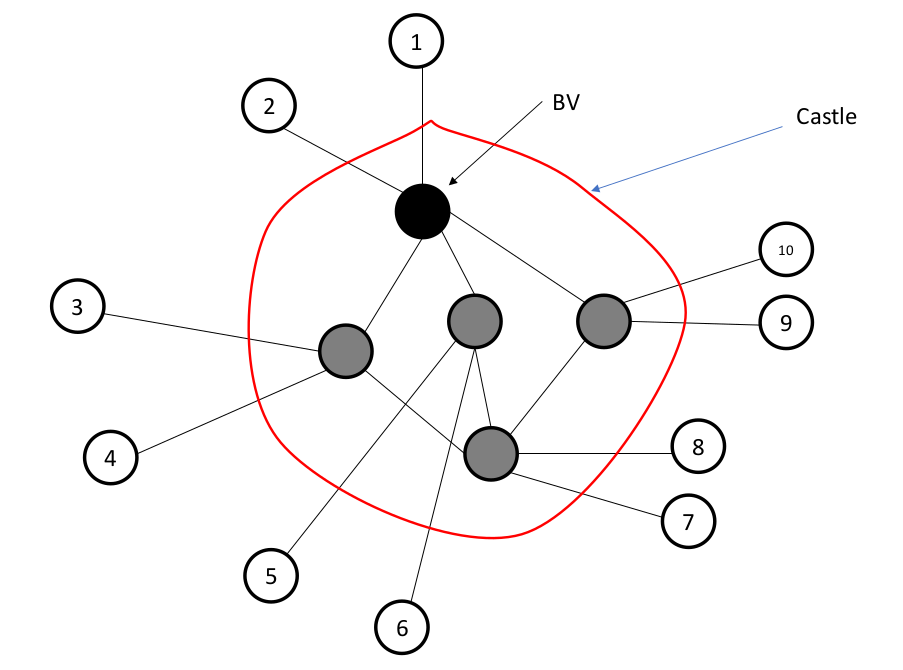
\includegraphics[width=3.5in]{figures/MultiCastleNode.png}
\caption{An example shows that if there is a BV in the castle, in some cases not all the guarding agents can receive a BV clone}\label{fig:MultiCastleNode}
\end{figure} 

So after the ``attacking" by the ``Attacking agent", the LA should execute a ``Double Patrol"   to check if there was a BV in this castle and to  locate it if there was.  We  now introduce the idea of   ``Double Patrol".
\begin{enumerate}
\item 
The LA first computes a route to traverse all the castle nodes, (say the route is $x_0\rightarrow x_1 \rightarrow\ldots, x_m$ assuming that there are $m$ nodes in the castle). In this first ``patrol" (see Fig.\ref{fig:FirstPatrol}), the LA first leaves a flag saying: ``First Patrol" and then moves to one castle node, it tells the SA residing in that castle node to collect the SAs residing in all its lower $SNR$ neighbours and finally moves to that castle node with all these collected SAs. Also, when the SA collects the agents  residing in the lower $SNR$ neighbours, it places a flag on that neighbour node saying: ``First Patrol". After the LA traverses all the castle nodes, it can easily know whether there is a BV in the castle: if there is no BV in the castle, then there should be one agent residing in every castle node and the LA would start the ``second patrol". Otherwise, there is a BV and its clones  have moved   to higher $SNR$ neighbours of this node. If the LA realizes that there is a BV, it stops traversing the remaining castle nodes.\\ 
%we know that in both situations, the LA should move back to the first castle node with the route $castle\_0\rightarrow castle\_1 \rightarrow\ldots, castle\_x$ and when it moves to every castle node, it should wait until all the guarding agents of that castle node being collected and then moves to the next castle node. When the LA moves back to the first castle node, the ``First Patrol" finishes. 

\begin{figure} [H]
  \centering 
  \ContinuedFloat
  \subfigure[$T_a$]{ 
    \label{fig:FirstPatrol1:a} %% label for first subfigure 
    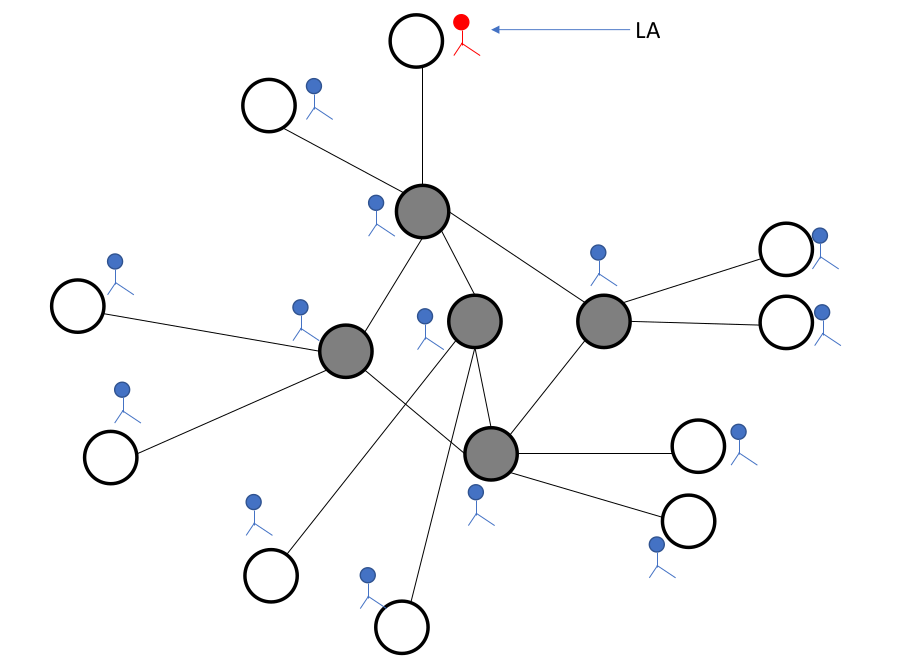
\includegraphics[width=2.5in]{figures/FirstPatrol1.png}} 
%  \hspace{1in} 
  \subfigure[$T_{a+1}$]{ 
    \label{fig:FirstPatrol2:b} %% label for second subfigure 
    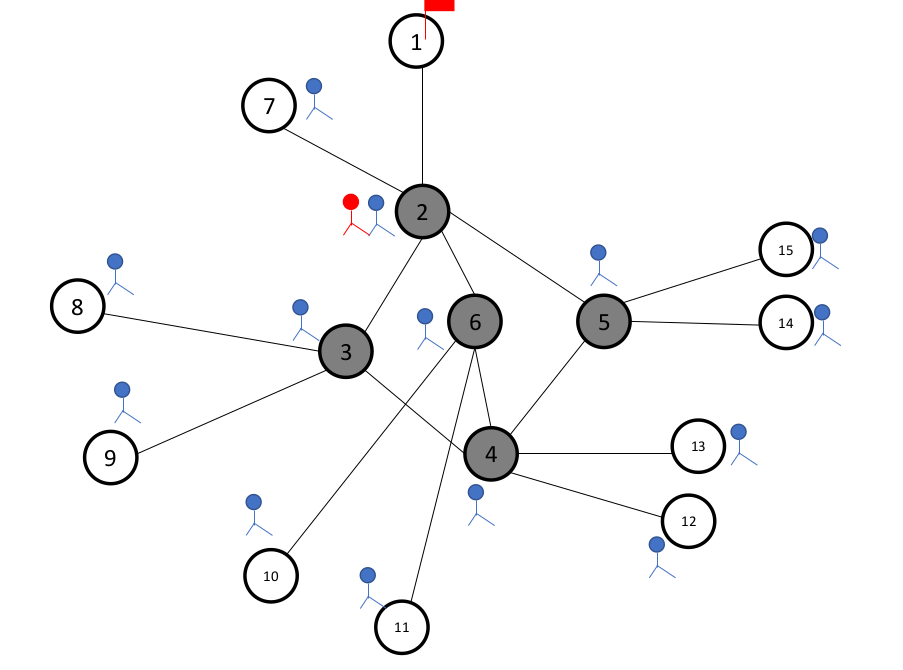
\includegraphics[width=2.5in]{figures/FirstPatrol2.png}}
    \hspace{1in} 
  \subfigure[$T_{a+2}$]{ 
    \label{fig:FirstPatrol3:c} %% label for second subfigure 
    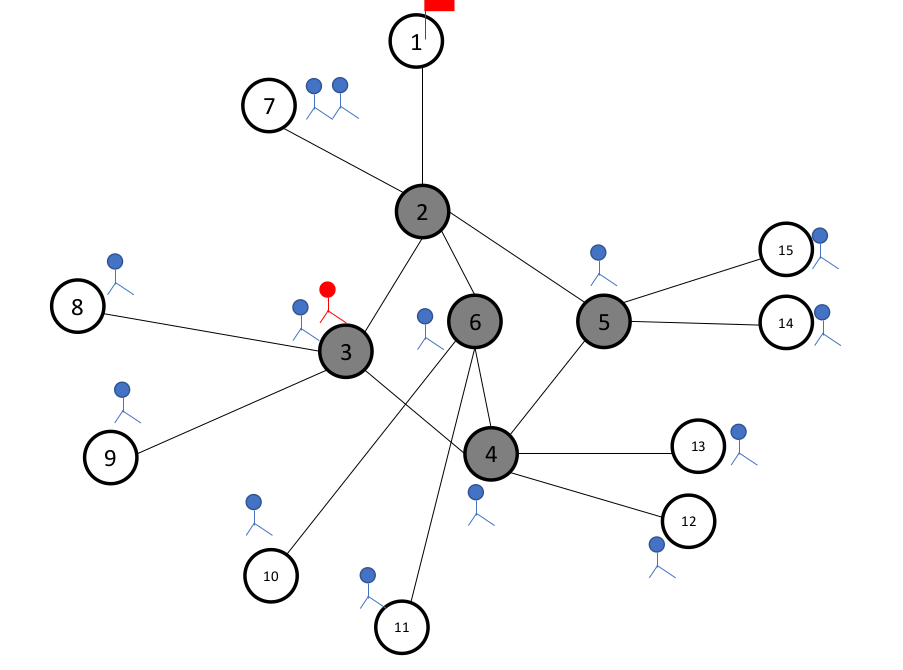
\includegraphics[width=2.5in]{figures/FirstPatrol3.png}}
%      \hspace{1in} 
  \subfigure[$T_{a+3}$]{ 
    \label{fig:FirstPatrol4:d} %% label for second subfigure 
    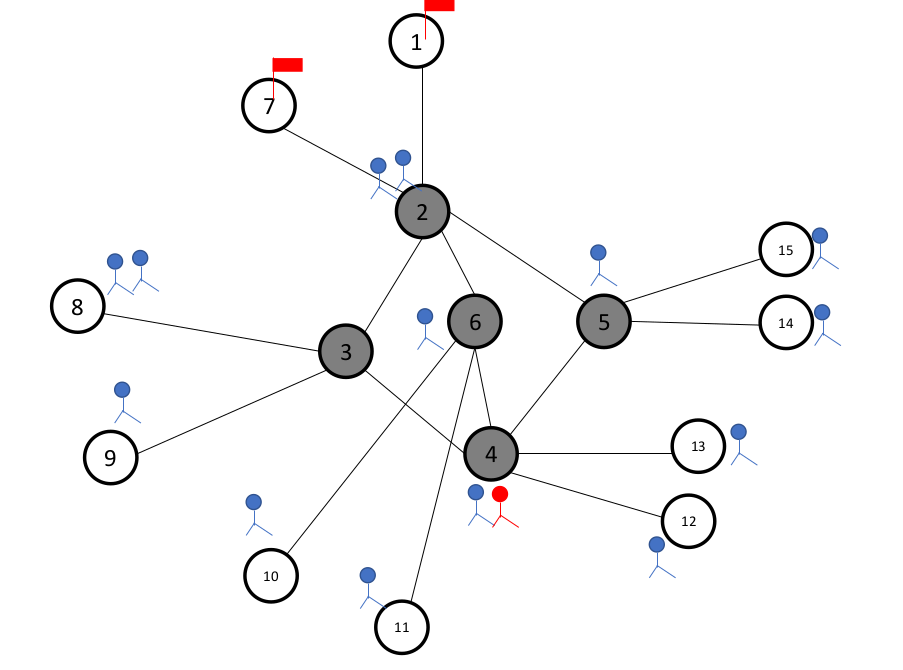
\includegraphics[width=2.5in]{figures/FirstPatrol4.png}}
      \hspace{1in} 
  \subfigure[$T_{a+4}$]{ 
    \label{fig:FirstPatrol5:e} %% label for second subfigure 
    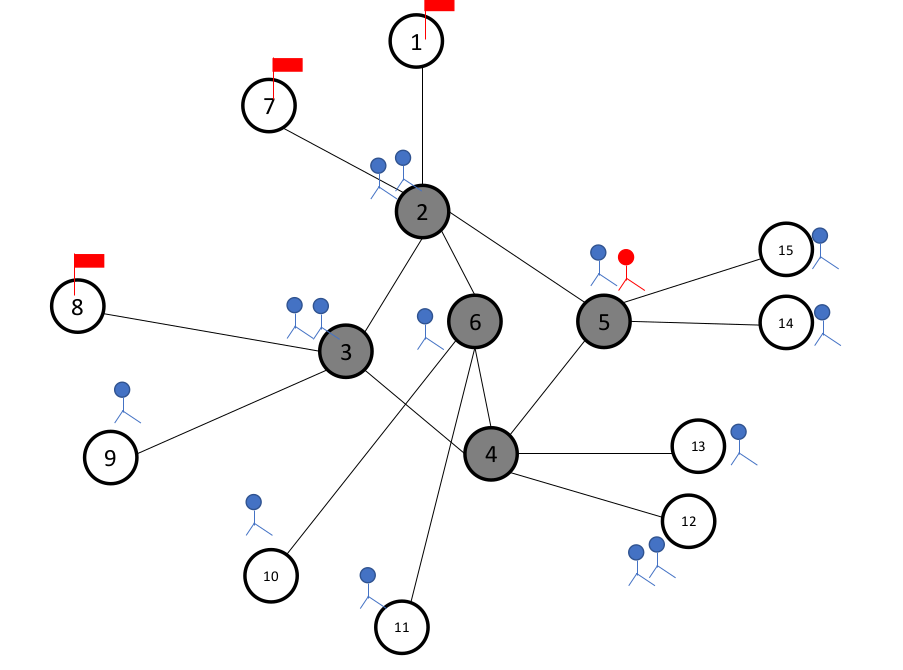
\includegraphics[width=2.5in]{figures/FirstPatrol5.png}}
     \subfigure[$T_{a+5}$]{ 
    \label{fig:FirstPatrol6:f} %% label for second subfigure 
    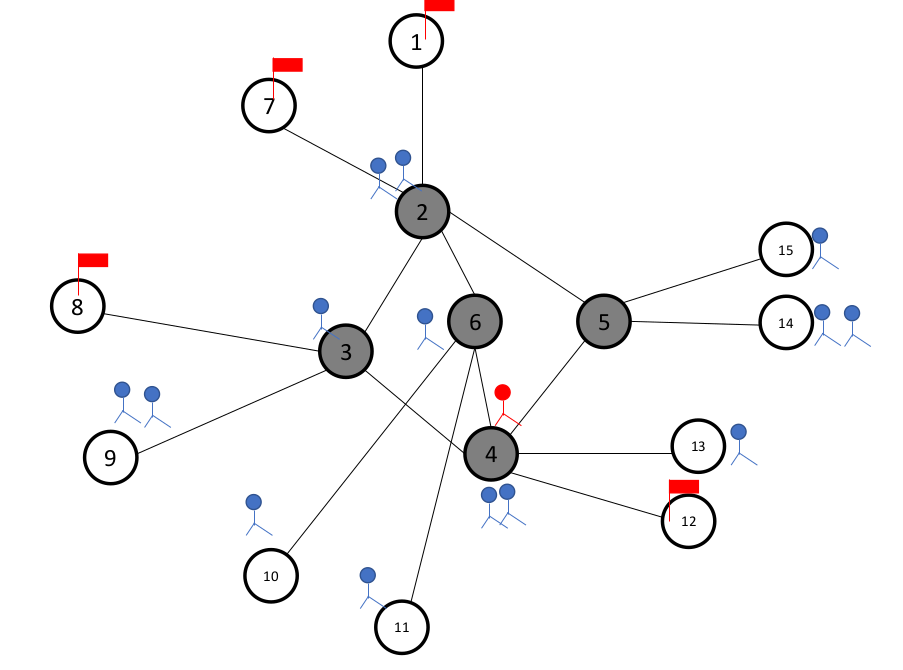
\includegraphics[width=2.5in]{figures/FirstPatrol6.png}}
  \caption{An example of  ``FirstPatrol"} 
  \label{fig:FirstPatrol} %% label for entire figure 
\end{figure}
\begin{figure} [H]
    
  \centering 
    \subfigure[$T_{a+6}$]{ 
    \label{fig:FirstPatrol7:g} %% label for first subfigure 
    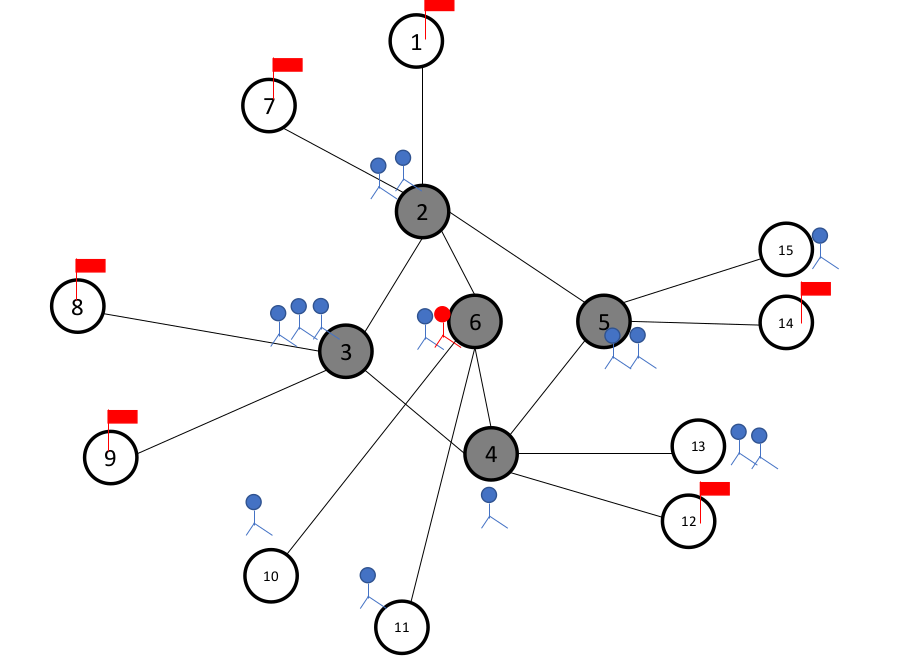
\includegraphics[width=2.3in]{figures/FirstPatrol7.png}} 
  \subfigure[$T_{a+7}$]{ 
    \label{fig:FirstPatrol8:h} %% label for second subfigure 
    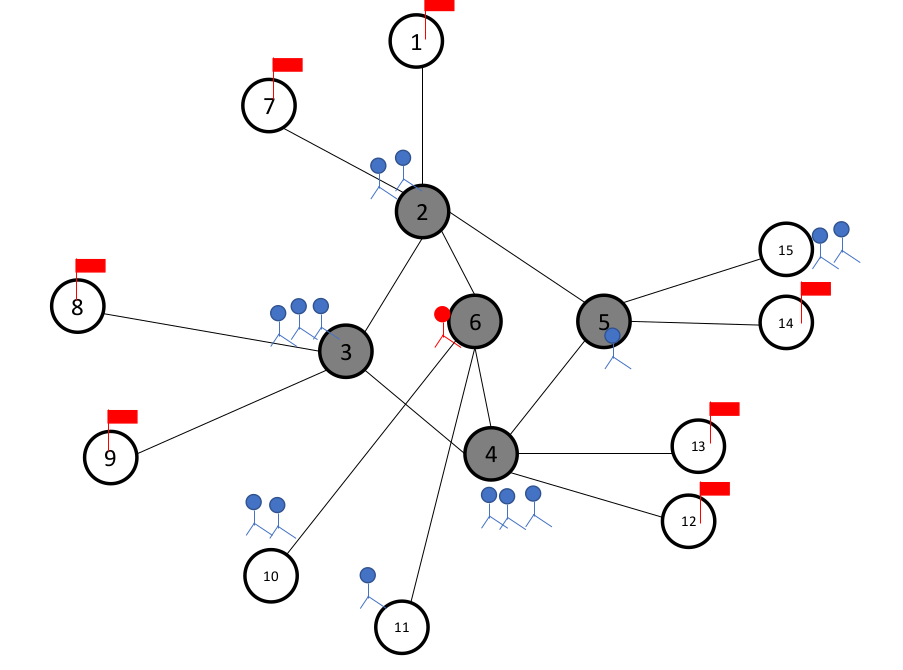
\includegraphics[width=2.3in]{figures/FirstPatrol8.png}}
    \hspace{1in} 
  \subfigure[$T_{a+8}$]{ 
    \label{fig:FirstPatrol9:i} %% label for second subfigure 
    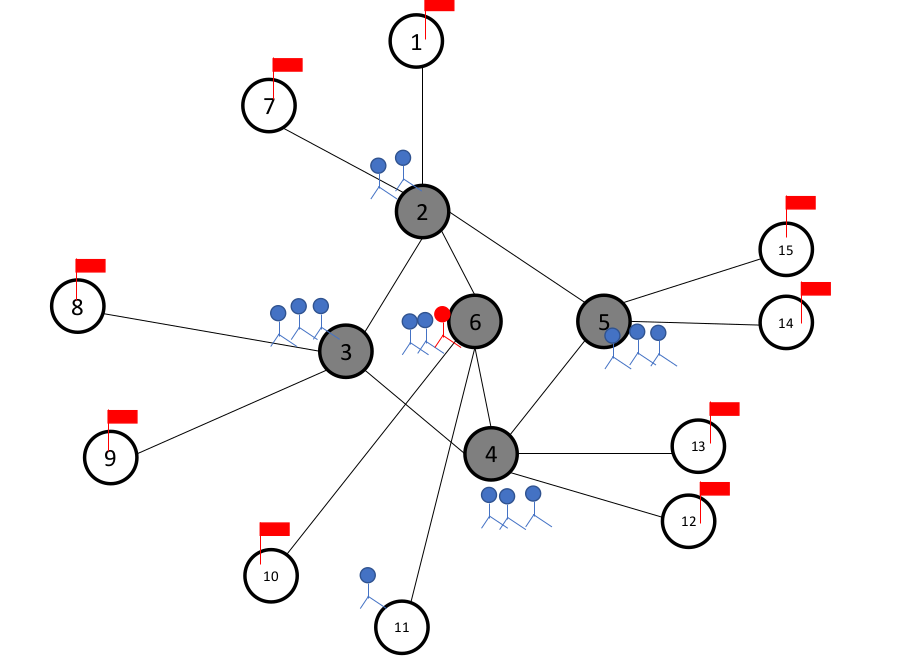
\includegraphics[width=2.3in]{figures/FirstPatrol9.png}}
  \subfigure[$T_{a+9}$]{ 
    \label{fig:FirstPatrol10:j} %% label for second subfigure 
    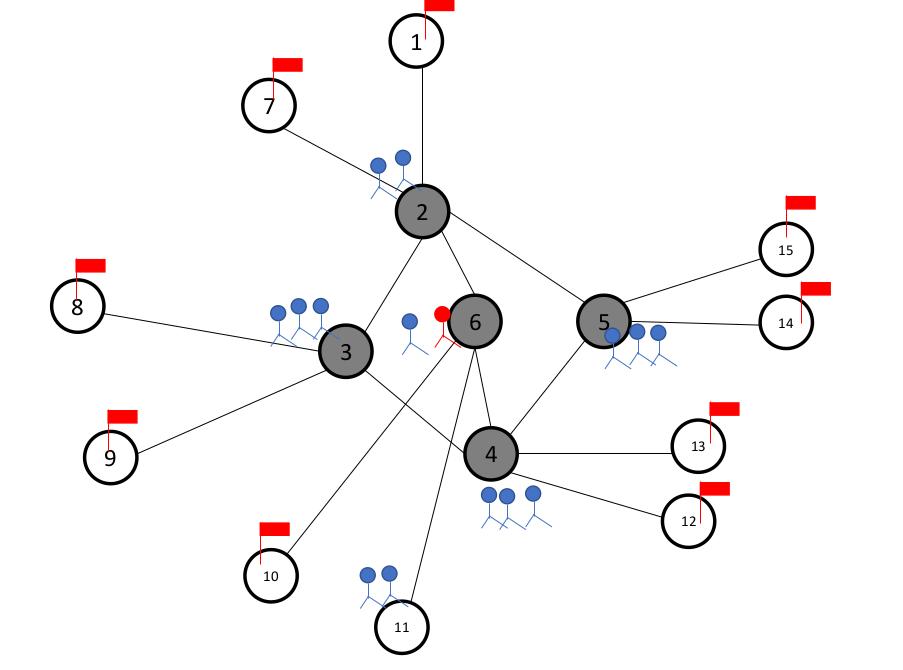
\includegraphics[width=2.3in]{figures/FirstPatrol10.png}}
      \hspace{1in} 
  \subfigure[$T_{a+10}$]{ 
    \label{fig:FirstPatrol11:k} %% label for second subfigure 
    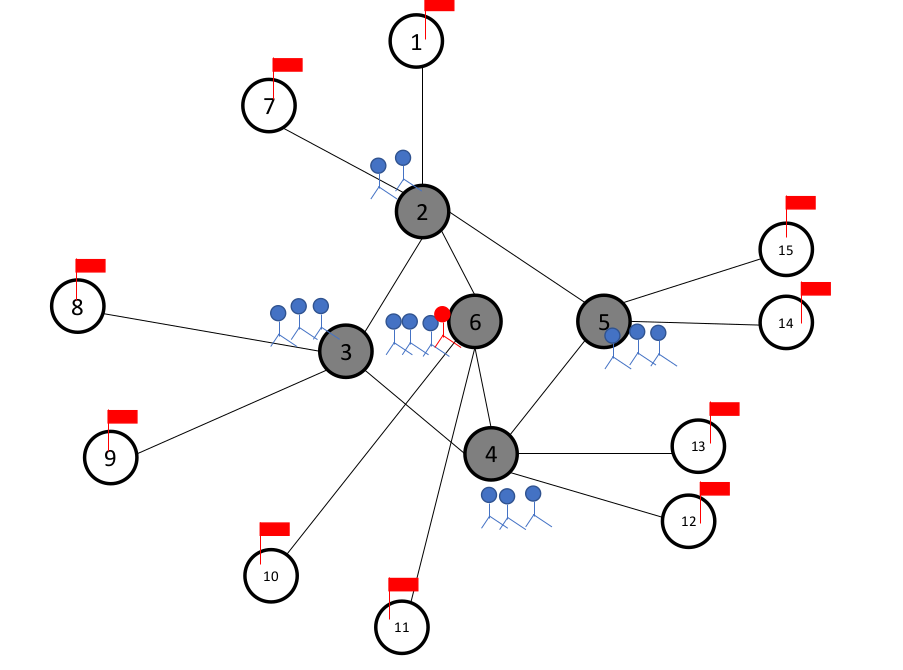
\includegraphics[width=2.5in]{figures/FirstPatrol11.png}}
  \caption{An example of  ``FirstPatrol" } 
  \label{fig:FirstPatrol} %% label for entire figure 
\end{figure}


\item 
After the first patrol,    if there is a BV the Elimination phase starts; otherwise,  the ``Second Patrol" starts. In the ``Second Patrol" the LA moves along the reverse route of  the ``First Patrol" which is $x_m \rightarrow x_{m-1} \rightarrow\ldots, x_0$.  While doing so,  it collects all the SAs in the castle node   and  it updates the information on the whiteboards on the castle nodes (if they have a whiteboard) saying that the castle is explored. \color{blue}what do you mean, if they have a whiteboard ? Are we assuming the whiteboard or not ?the whiteboards are placed on node with more than two neighbours, some of the castles may have less or equal to two neighbours \color{black}
\end{enumerate}  
After the ``Second Patrol", the status of this agent group changes into ``Finding-Castle" again. 

(2) From ``Finding-Castle" to ``Waiting-in-Line"

When the status of the agent group changes into ``Waiting-in-Line", then it means that the  LA in that agent group cannot find an available castle but there are still castles unexplored in the graph. At this time, the LA    chooses a castle marked ``under exploration" and moves there with its agent group. When the   group arrives in one of the lower $SNR$ neighbours of that castle (the ``Guarding Node")  three situations may happen:
\begin{enumerate}
\item Case 1: The agent group arrives at the Guarding node finding that no SA(s) and no flag in that  Guarding Node. In this situation, the agent group who is expected to attack this castle may not have yet arrived to this castle or may not have  finished the arrangement of the SAs. Then the agent group should wait at that guarding node until there is an SA and   follow  the instruction of Case 2 when this happens.  

\item Case 2: The agent group arrives at the Guarding node finding at least one SA. In this situation, it means that the agent group who is expected to attack the castle has finished arranging the SAs but has not finished the ``First Patrol". So, this agent group stays with the SA until the SA is called by another SA and moves into the castle. After moving into the castle node, the agent group should wait for the LA of the agent group that is attacking the castle, to move to this castle node again because at this time the LA would update the situation in the castle: whether there is a BV or not. If there is a BV in the castle, then the agent group that is waiting in the castle node ends its exploration phase and start the elimination phase; otherwise,   the status of this agent group changes into ``Finding-Castle".

\item Case 3:The agent group arrives at the Guarding node and finds that there is a flag. This means that the LA of the agent group who is excepted to attack the castle is doing (or has finished) the ``First Patrol", or it is doing the   ``Second Patrol". In this situation, the agent group moves into the castle node which is connected to the guarding node   and wait  for the LA of the attacking  group  to move to this castle node again. As in Case 2, this agent group  knows   if there is a BV in the castle:  if there is a BV, then the agent group starts the elimination phase, otherwise its status  changes into ``Finding-Castle".
\end{enumerate}


\subsection{ Elimination Phase}

When the BV is triggered,   the location of the BVs can be in a castle or outside the castles. In both situation, the lower $SNR$ neighbours of the BV node or the castle containing the BV have been guarded by the agents. In other words, when the BV is triggered, only the clones spreading to the higher $SNR$ neighbours %(say there are $y$ such nodes) 
survive and their locations are exposed. Also, the locations of all the neighbours of these new formed BVs are exposed. 

So, the LA computes the routes from where it resides to all the nodes needing guarding, including both  the lower and the higher $SNR$ neighbours   (Surrounding Nodes). If the location of the original BV is outside the castle, then all the SAs stay  with the LA, so the LA simply sends the SAs to these Surrounding Nodes. If the original BV is in the castle, then after the  ``Double Patrol", the LA knows the location of the original BV, so it computes the routes from where it resides to all the Surrounding Nodes and send the SAs to them (note that all the SAs are with the LA after the  ``Double Patrol"). Also note that since the graph is biconnected, there is always a route to reach the surrounding node bypassing the new formed BV nodes. 
\color{blue}
(Yes, we have this assumption, I add this assumption at the beginning  (marking blue) ) 
Actually, a single node cannot disconnect, but multiple nodes could (i.e., the original BV and its clones).
\color{black}
Assuming that there are $k$ higher $SNR$ neighbours of the original BV, then   the LA sends another $k$ agents to the new formed BV nodes and permanently destroy the BVs.
   


  









































 